\documentclass[11pt,a4paper]{article}
\usepackage[utf8]{inputenc}
\usepackage[spanish]{babel}
\usepackage{amsmath}
\usepackage{amsfonts}
\usepackage{amssymb}

\usepackage{hyperref}
\usepackage{graphicx}
\usepackage{geometry}
\usepackage{apacite}

\usepackage{listings}
\usepackage{xcolor}

\newgeometry{left=3cm, right=3cm, top=2.5cm, bottom=2.5cm}

\definecolor{codegreen}{rgb}{0,0.6,0}
\definecolor{codegray}{rgb}{0.5,0.5,0.5}
\definecolor{codepurple}{rgb}{0.58,0,0.82}
\definecolor{backcolour}{rgb}{0.95,0.95,0.92}

\lstdefinestyle{mystyle}{
	backgroundcolor=\color{backcolour},   
	commentstyle=\color{codegreen},
	keywordstyle=\color{magenta},
	numberstyle=\tiny\color{codegray},
	stringstyle=\color{codepurple},
	basicstyle=\ttfamily\footnotesize,
	breakatwhitespace=false,         
	breaklines=true,                 
	captionpos=b,                    
	keepspaces=true,                 
	numbers=left,                    
	numbersep=5pt,                  
	showspaces=false,                
	showstringspaces=false,
	showtabs=false,                  
	tabsize=2
}

\begin{document}
\begin{titlepage}
\centering


{\bfseries\LARGE UNIVERSIDAD NACIONAL DEL ALTIPLANO\par}
{\scshape\LARGE Facultad de Ingeniería Mecánica Eléctrica, Electrónica y Sistemas\par}
{\scshape\LARGE Escuela Profesional de Ingeniería de Sistemas\par}
\vspace{1cm}
{
\includegraphics[width=0.5\textwidth]{images/1-unap.png}\par}
\vspace{0.5cm}
{\bfseries\LARGE EVALUACIÓN DE PROGRAMACIÓN ORIENTADA A OBJETOS EN C++\par}
\vspace{1cm}
{\LARGE Docente: Mg. Aldo Hernan Zanabria Galvez \par}
{\LARGE Alumno: Yoel Nhelio Canaza Chagua \par}
\vspace{1cm}
{\LARGE Curso: \par}
{\LARGE Programación Orientada a Objetos II \par}
\vspace{1cm}
{\LARGE CICLO III – SEMESTRE 2023 – II \par}
{\LARGE PUNO, PERÚ \par}
{\LARGE 2023 \par}


\end{titlepage}

\section{Ejercicio 6. DIC04}
\subsection{1.a Especifica qué pasará en los siguientes casos, suponiendo que propio() está sobreescrito en las clases derivadas}
\begin{lstlisting}[language=C++, style=mystyle, caption={6-DIC04}]
#include <iostream>

using namespace std;

class Barco
{
public:
    Barco();
    virtual ~Barco();
    virtual void propio() const;
    void ver();
    
    static int obtenerNumeroBarcos();
protected:
    static int numeroBarcos;
};

int Barco::numeroBarcos = 0;

Barco::Barco()
{
    cout << "Creando barco... " << endl;
    numeroBarcos += 1;
}

Barco::~Barco()
{
    cout << "Eliminando barco... " << endl;
    numeroBarcos -= 1;
}

void Barco::propio() const
{
    cout << "BARCO: Se ha llamado a la funcion propio()" << endl;
}

int Barco::obtenerNumeroBarcos()
{
    return numeroBarcos;
}

void Barco::ver()
{
    cout << "Se ha llamado a la funcion ver()" << endl;
}



class Submarino : public Barco
{
public:
    Submarino() {}
    void propio() const override;

protected:

};

void Submarino::propio() const
{
    cout << "SUBMARINO: Se ha llamado a la funcion propio() sobreescrita por la clase derivada Submarino" << endl;
}



class Destructor : public Barco
{
public:
    Destructor() {}
    void propio() const override;
protected:
};

void Destructor::propio() const{
    cout << "DESTRUCTOR: Se ha llamado a la funcio1n propio() sobreescrita por la clase derivada Destructor" << endl;
}

int main()
{
    // 1.a Especifica que pasara en los siguientes casos, suponiendo que propio() esta sobreescrito en las clases derivadas
    // a
    Barco* a = new Barco();
    a->propio();
    a->ver();
    cout << endl;
    // b
    Barco* b = new Submarino();
    b->propio();
    b->ver();
    cout << endl;

    // c
    Barco* c[] = {new Barco(), new Submarino()};
    c[0]->propio();
    c[1]->propio();
    c[0]->ver();
    cout << endl;

    // d
    Barco* d[] = {new Destructor(), new Submarino()};
    d[0]->propio();
    d[1]->propio();
    cout << endl;

    // e: supongamos que anadimos ver() heredado del padre tanto en submarino como en destructor;

    Barco* e[] = {new Destructor(), new Submarino()};
    ((Destructor *)e[0])->ver();
    ((Submarino *)e[1])->ver();
    e[0]->ver();
    e[1]->ver();
    cout << endl;



}
\end{lstlisting}

{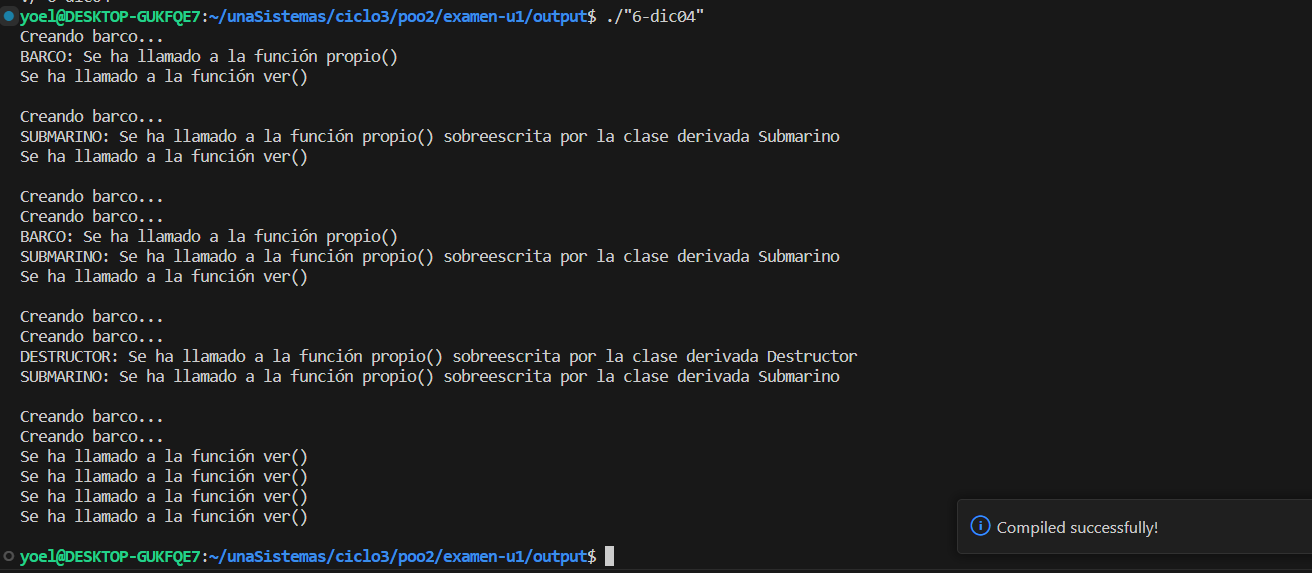
\includegraphics[width=1\textwidth]{images/1-compilado.png}\par}

\subsubsection{a. }
Se crea un objeto a se la clase Barco y se llama a las funciones propio y ver, como estas funciones pertenecen a la clase base se muestran las funciones sin modificar.
\subsubsection{b. }
Se crea un objeto a se la clase Submarino y se llama a las funciones propio y ver, como estas funciones pertenecen a la clase derivada Submarino se muestra la funcion modificada de subamarino.
\subsubsection{c. }
Se crea un array de objetos a se la clase Barco y Submarino y se llama a las funciones propio y ver, como funciones pertenecen a la clase derivada Submarino se muestra la funcion modificada de subamarino. Sin embargo en el caso del objeto de la clase Barco, se muestra la función por defecto
\subsubsection{d. }
Se crea un array de objetos a se la clase Barco y Submarino y se llama a las funciones propio y ver, como funciones pertenecen a clases derivadas, se muestran las implementaciones que estos tienen para dichas funciones.

\subsection{1.b Supongamos que la asignatura del método propio es la siguiente:  virtual void Barco::propio()=0;}

{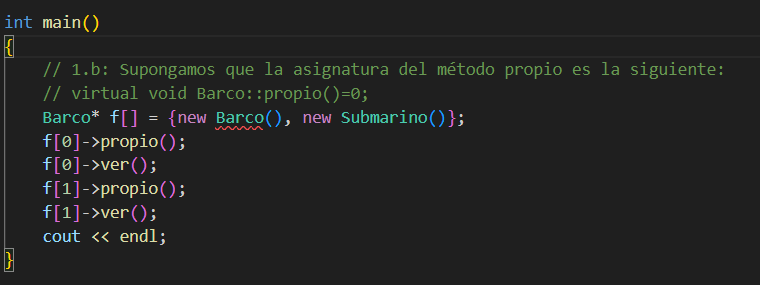
\includegraphics[width=1\textwidth]{images/2-codigo.png}\par}
Si agregamos el anterior codigo teniendo void Barco::propio()=0; obtendremos el siguiente error:

{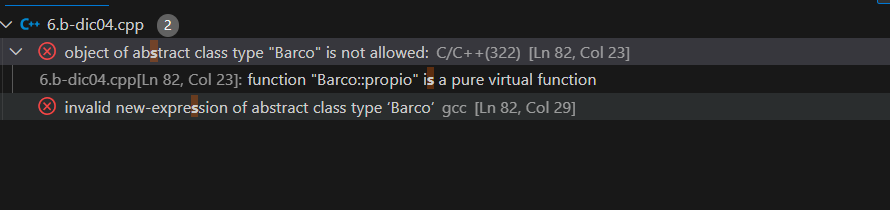
\includegraphics[width=1\textwidth]{images/3-error.png}\par}


Este error generalmente se produce cuando intentamos crear una instancia (un objeto) de una clase abstracta directamente. Las clases abstractas son aquellas que tienen al menos una función virtual pura (una función virtual que se declara con = 0 y no se implementa en la clase base). No se pueden crear instancias de clases abstractas, ya que no tienen una implementación completa de todas sus funciones virtuales.






\section{12 SEP06: Define una funcion genérica llamada 'Intercambio que permita intercambiar el valor de dos objetos del mismo tipo. Indica qué restricciones debe cumplir el tipo de los objetos para poder usar a función de intercambio con ellos
}



\begin{lstlisting}[language=C++, style=mystyle, caption={12 SEPT06}]
//Ejercicio 12-sep06
//Ejercicio 12-sep06
#include <iostream>
#include <string>

using namespace std;


class Carta {
public:
    Carta(string valor, string palo) : valor_(valor), palo_(palo) {}

 
    friend ostream& operator<<(ostream& os, const Carta& carta) {
        os << "Carta: " << carta.valor_ << " de " << carta.palo_;
        return os;
    }

private:
    string valor_;
    string palo_;
};

template <typename T>
void Intercambio(T &a, T &b) {
    T temp = a;
    a = b;
    b = temp;
}

int main() {
    Carta As1("As", "Corazones");
    Carta As2("As", "Treboles");

    cout << "Antes del intercambio: " << endl;
    cout << As1 << endl;
    cout << As2 << endl; 


    Intercambio(As1, As2);

    cout << "Despues del intercambio: " << endl;
    cout << As1 << endl; 
    cout << As2 << endl; 

    return 0;
}


\end{lstlisting}

Los objetos deben ser del mismo tipo


{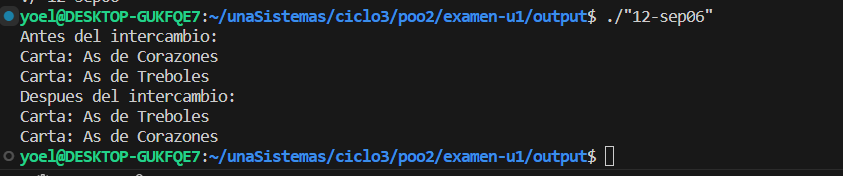
\includegraphics[width=1\textwidth]{images/4-compilado.png}\par}





\end{document}